\chapter{System Design}
\label{ch:system_design}

\section{Introduction}

This chapter presents the comprehensive system design for the machine learning and IoT-based traffic management system. The design encompasses the overall system architecture, individual component specifications, data flow mechanisms, and integration strategies. The system is designed to address the unique challenges of traffic management in Dhaka city while providing scalable and robust performance for real-world deployment.

\section{System Architecture Overview}

\subsection{High-Level Architecture}

The proposed traffic management system follows a hierarchical architecture with three main layers:

\begin{enumerate}
    \item \textbf{Data Acquisition Layer}: Responsible for capturing and preprocessing real-time traffic data
    \item \textbf{Processing Layer}: Handles machine learning inference, traffic analysis, and decision making
    \item \textbf{Control Layer}: Manages traffic signal control and hardware interface
\end{enumerate}

\begin{figure}[h]
    \centering
    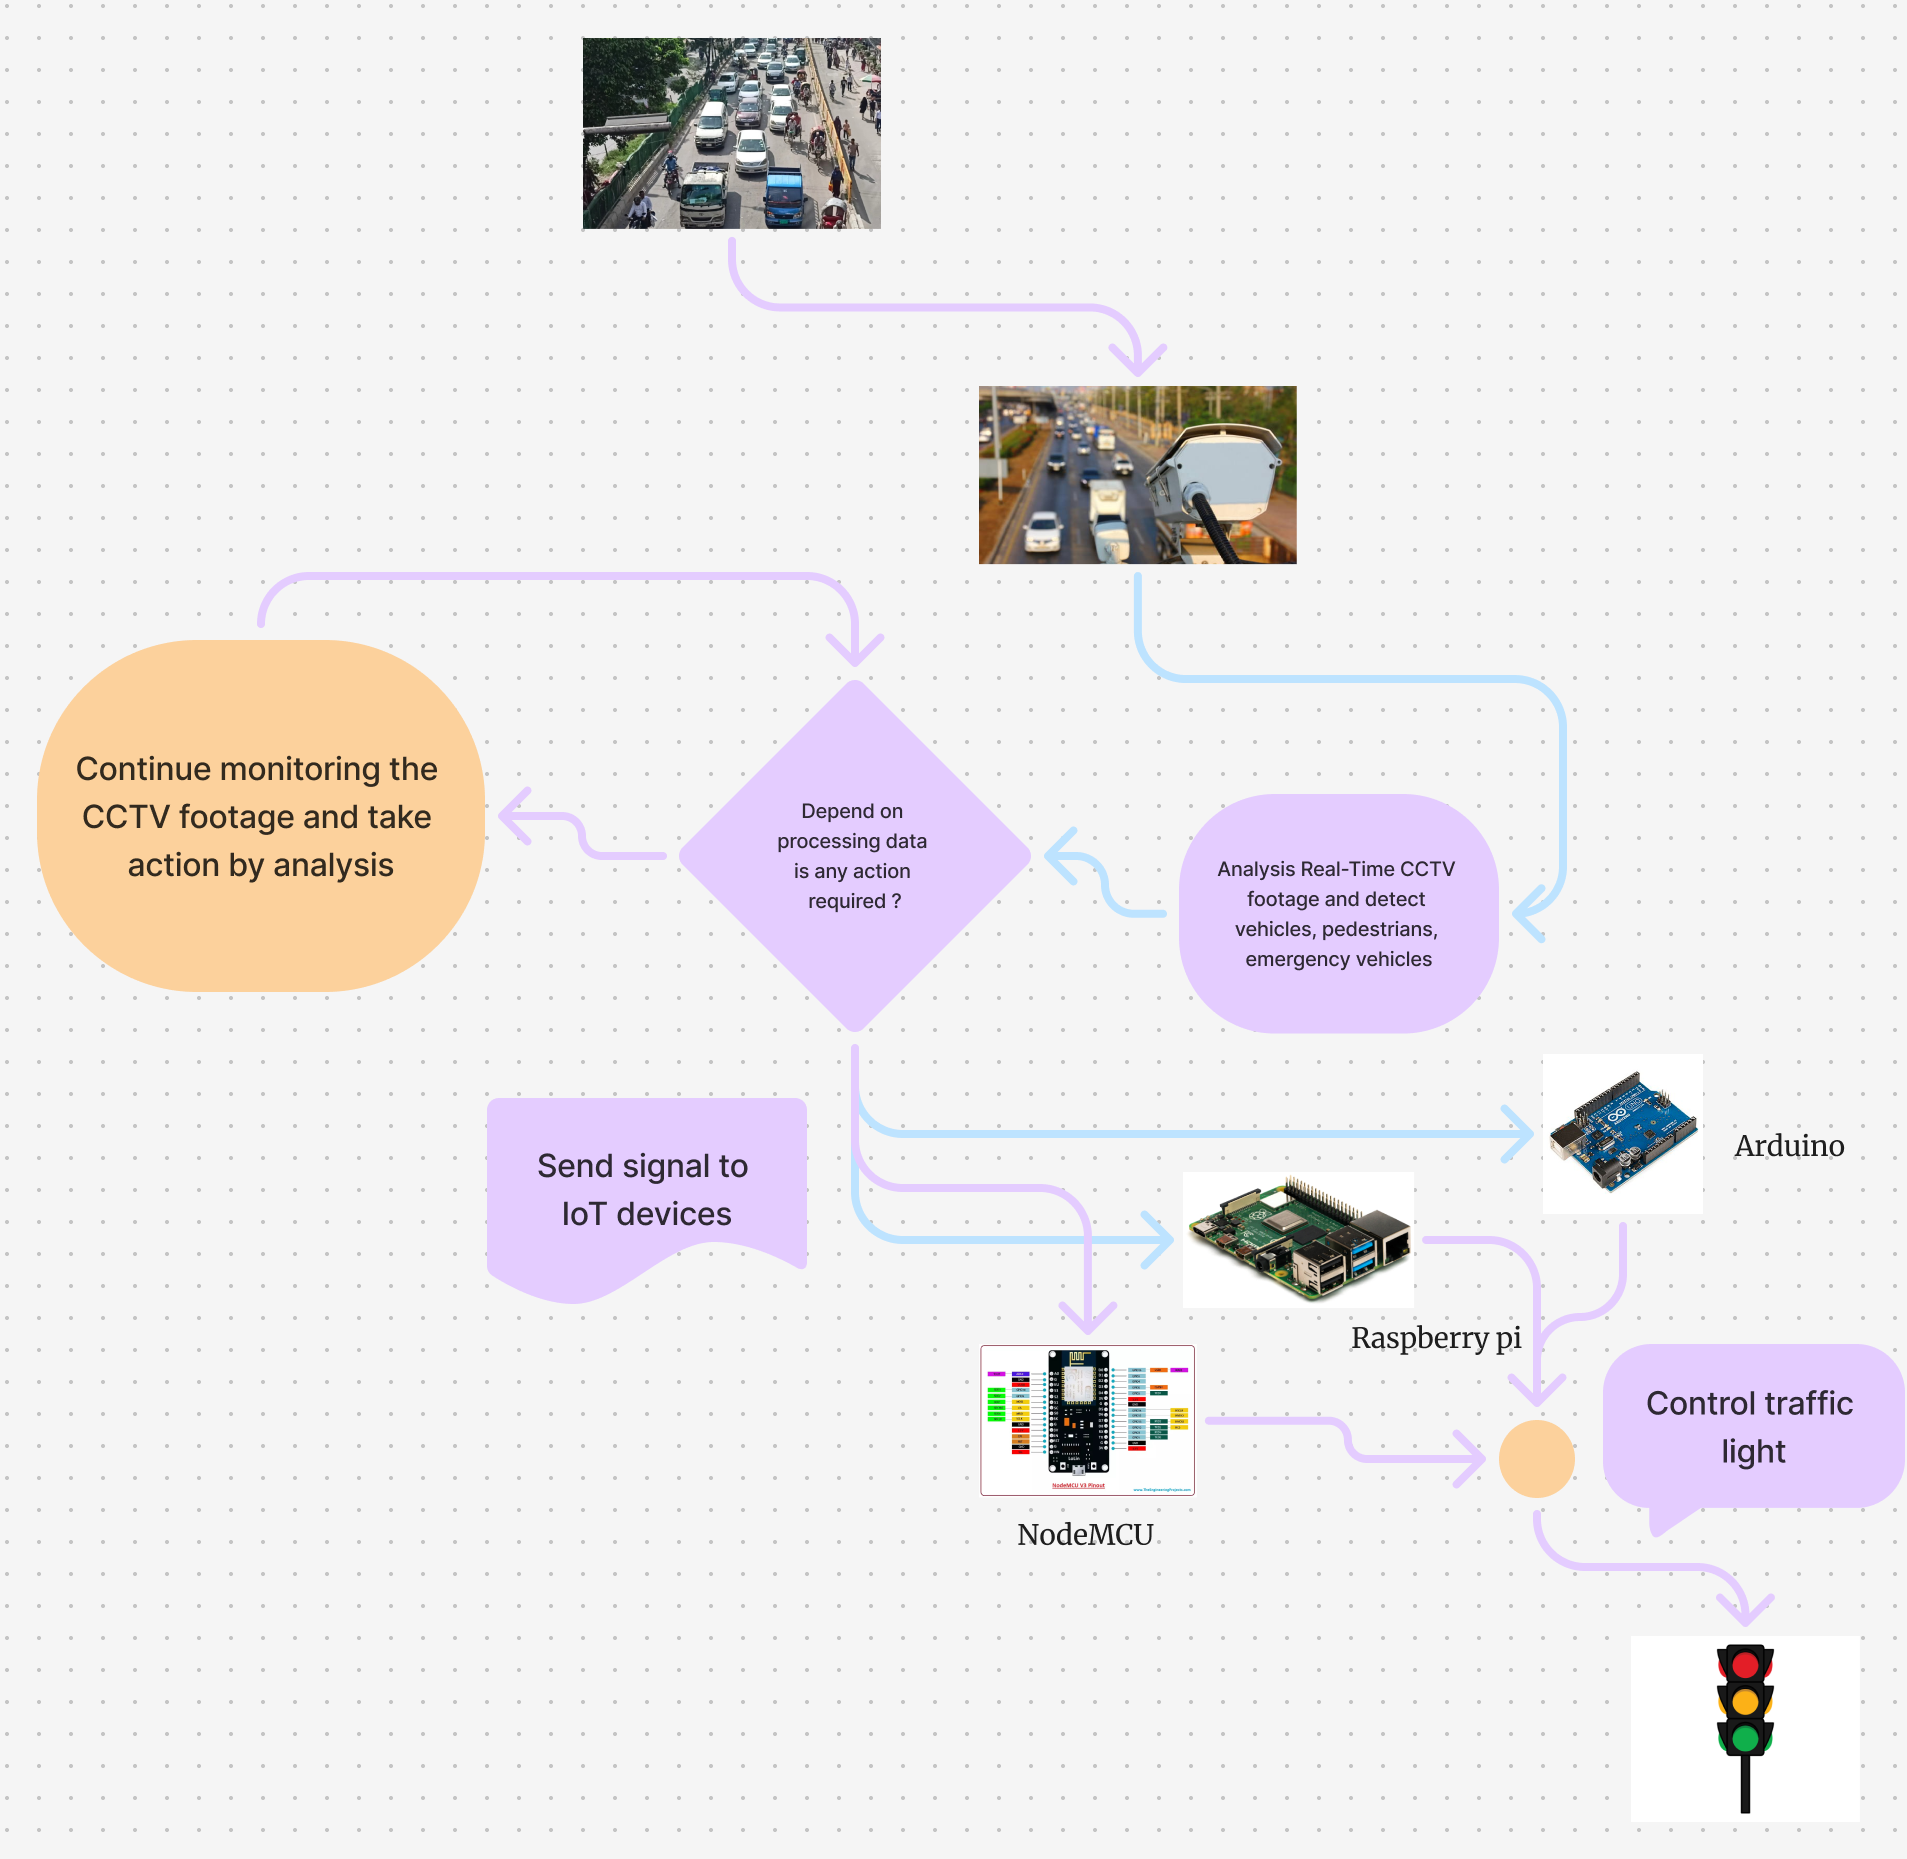
\includegraphics[width=0.8\textwidth]{figures/6_.png}
    \caption{Overall System Architecture}
    \label{fig:system_architecture}
\end{figure}

\subsection{System Components}

The system comprises six main components:

\begin{enumerate}
    \item \textbf{Video Capture Module}: Real-time video acquisition from CCTV cameras
    \item \textbf{Object Detection Module}: YOLOv11-based vehicle and pedestrian detection
    \item \textbf{Traffic Analysis Module}: Traffic flow analysis and congestion assessment
    \item \textbf{Decision Engine}: Traffic signal control logic and emergency prioritization
    \item \textbf{Hardware Interface Module}: Connection to physical traffic signal systems
    \item \textbf{Monitoring and Reporting Module}: System status monitoring and performance reporting
\end{enumerate}

\section{Data Acquisition Layer}

\subsection{Video Capture Module}

The video capture module serves as the primary interface between the physical traffic environment and the digital processing system.

\subsubsection{Camera Specifications}

The system utilizes high-resolution cameras with the following specifications:

\begin{table}[h]
\centering
\caption{Camera Specifications}
\begin{tabular}{|l|l|}
\hline
\textbf{Parameter} & \textbf{Specification} \\
\hline
Resolution & 1920x1080 pixels (Full HD) \\
Frame Rate & 30 FPS \\
Video Format & H.264/H.265 \\
Field of View & 90-120 degrees \\
Night Vision & Infrared capability \\
Weather Resistance & IP66 rating \\
Power Requirements & 12V DC, 2A \\
\hline
\end{tabular}
\end{table}

\subsubsection{Camera Placement Strategy}

Strategic camera placement is crucial for optimal system performance:

\begin{enumerate}
    \item \textbf{Height}: 4-6 meters above ground level
    \item \textbf{Angle}: 15-30 degrees downward angle
    \item \textbf{Coverage}: Complete intersection coverage with minimal blind spots
    \item \textbf{Positioning}: Multiple cameras per intersection for comprehensive coverage
    \item \textbf{Redundancy}: Backup cameras for critical intersections
\end{enumerate}

\subsection{Data Preprocessing Module}

The preprocessing module prepares raw video data for machine learning inference:

\subsubsection{Frame Extraction}

\begin{algorithmic}[1]
\STATE \textbf{Input:} Video stream from camera
\STATE \textbf{Output:} Processed frames for inference
\STATE 
\WHILE{video\_stream\_active}
    \STATE frame = capture\_frame()
    \IF{frame\_quality\_check(frame)}
        \STATE processed\_frame = preprocess(frame)
        \STATE send\_to\_detection\_module(processed\_frame)
    \ENDIF
\ENDWHILE
\end{algorithmic}

\subsubsection{Image Enhancement}

The preprocessing pipeline includes:

\begin{enumerate}
    \item \textbf{Noise Reduction}: Gaussian filtering for noise removal
    \item \textbf{Contrast Enhancement}: Histogram equalization for better visibility
    \item \textbf{Color Correction}: Automatic white balance adjustment
    \item \textbf{Resolution Standardization}: Resizing to standard input dimensions
    \item \textbf{Format Conversion}: Converting to appropriate format for YOLO inference
\end{enumerate}

\section{Processing Layer}

\subsection{Object Detection Module}

The object detection module is the core component responsible for identifying and classifying vehicles and pedestrians in real-time.

\subsubsection{YOLOv11 Implementation}

The YOLOv11 model is implemented with the following architecture:

\begin{table}[h]
\centering
\caption{YOLOv11 Model Configuration}
\begin{tabular}{|l|l|}
\hline
\textbf{Parameter} & \textbf{Value} \\
\hline
Model Size & YOLOv11m (Medium) \\
Input Resolution & 640x640 pixels \\
Number of Classes & 21 (vehicles + pedestrians) \\
Confidence Threshold & 0.5 \\
NMS Threshold & 0.45 \\
Batch Size & 1 (real-time inference) \\
\hline
\end{tabular}
\end{table}

\subsubsection{Detection Pipeline}

The detection pipeline operates as follows:

\begin{algorithmic}[1]
\STATE \textbf{Input:} Preprocessed frame
\STATE \textbf{Output:} Detection results with bounding boxes and classifications
\STATE 
\STATE frame\_tensor = convert\_to\_tensor(frame)
\STATE predictions = yolo\_model(frame\_tensor)
\STATE detections = non\_max\_suppression(predictions)
\STATE 
\FOR{each detection in detections}
    \STATE bbox = detection.bbox
    \STATE class\_id = detection.class\_id
    \STATE confidence = detection.confidence
    \STATE 
    \IF{confidence > threshold}
        \STATE add\_to\_results(bbox, class\_id, confidence)
    \ENDIF
\ENDFOR
\STATE 
\STATE RETURN detection\_results
\end{algorithmic}

\subsection{Traffic Analysis Module}

The traffic analysis module processes detection results to extract meaningful traffic information.

\subsubsection{Vehicle Counting and Classification}

\begin{enumerate}
    \item \textbf{Lane Assignment}: Assigning detected vehicles to specific lanes
    \item \textbf{Vehicle Counting}: Counting vehicles per lane and total intersection
    \item \textbf{Classification}: Categorizing vehicles into regular and emergency types
    \item \textbf{Tracking}: Maintaining vehicle trajectories for flow analysis
    \item \textbf{Speed Estimation}: Calculating average vehicle speeds
\end{enumerate}

\subsubsection{Traffic Flow Analysis}

The system performs comprehensive traffic flow analysis:

\begin{algorithmic}[1]
\STATE \textbf{Input:} Detection results from multiple frames
\STATE \textbf{Output:} Traffic flow statistics
\STATE 
\STATE Initialize lane\_counts = [0, 0, 0, 0]  \COMMENT{North, South, East, West}
\STATE Initialize wait\_times = [0, 0, 0, 0]
\STATE Initialize emergency\_vehicles = []
\STATE 
\FOR{each detection in current\_detections}
    \STATE lane\_id = assign\_lane(detection.bbox)
    \STATE lane\_counts[lane\_id] += 1
    \STATE 
    \IF{detection.class\_id in emergency\_classes}
        \STATE emergency\_vehicles.append(detection)
    \ENDIF
\ENDFOR
\STATE 
\STATE congestion\_level = calculate\_congestion(lane\_counts)
\STATE priority\_scores = calculate\_priority\_scores(lane\_counts, wait\_times)
\STATE 
\STATE RETURN traffic\_statistics
\end{algorithmic}

\subsection{Decision Engine}

The decision engine is responsible for traffic signal control logic and emergency vehicle prioritization.

\subsubsection{Emergency Vehicle Prioritization}

The emergency vehicle prioritization algorithm:

\begin{algorithmic}[1]
\STATE \textbf{Input:} Current traffic state and emergency vehicle detections
\STATE \textbf{Output:} Signal control commands
\STATE 
\STATE emergency\_detected = False
\STATE priority\_lane = None
\STATE 
\FOR{each emergency\_vehicle in emergency\_vehicles}
    \STATE lane = get\_vehicle\_lane(emergency\_vehicle)
    \STATE distance = estimate\_distance(emergency\_vehicle)
    \STATE 
    \IF{distance < emergency\_activation\_threshold}
        \STATE emergency\_detected = True
        \STATE priority\_lane = lane
        \STATE BREAK
    \ENDIF
\ENDFOR
\STATE 
\IF{emergency\_detected}
    \STATE activate\_emergency\_mode(priority\_lane)
\ELSE
    \STATE apply\_normal\_traffic\_control()
\ENDIF
\end{algorithmic}

\subsubsection{Normal Traffic Control Algorithm}

For normal traffic conditions, the system uses a Weighted Job First (WJF) scheduling algorithm:

\begin{algorithmic}[1]
\STATE \textbf{Input:} Lane traffic densities and wait times
\STATE \textbf{Output:} Next lane to activate
\STATE 
\STATE Initialize max\_score = 0
\STATE Initialize selected\_lane = None
\STATE 
\FOR{each lane in [North, South, East, West]}
    \STATE vehicle\_count = get\_vehicle\_count(lane)
    \STATE wait\_time = get\_wait\_time(lane)
    \STATE starvation\_factor = calculate\_starvation\_factor(wait\_time)
    \STATE 
    \STATE score = (vehicle\_count × vehicle\_weight) + (wait\_time × time\_weight) + starvation\_factor
    \STATE 
    \IF{score > max\_score}
        \STATE max\_score = score
        \STATE selected\_lane = lane
    \ENDIF
\ENDFOR
\STATE 
\STATE RETURN selected\_lane
\end{algorithmic}

\section{Control Layer}

\subsection{Hardware Interface Module}

The hardware interface module connects the software system to physical traffic signal infrastructure.

\subsubsection{Microcontroller Integration}

The system supports multiple microcontroller platforms:

\begin{table}[h]
\centering
\caption{Supported Microcontroller Platforms}
\begin{tabular}{|l|l|l|}
\hline
\textbf{Platform} & \textbf{Specifications} & \textbf{Use Case} \\
\hline
Arduino Uno & 8-bit, 32KB Flash & Basic signal control \\
Arduino Mega & 8-bit, 256KB Flash & Extended functionality \\
Raspberry Pi 4 & 64-bit, 4GB RAM & Advanced processing \\
NodeMCU & 32-bit, WiFi enabled & IoT connectivity \\
\hline
\end{tabular}
\end{table}

\subsubsection{Signal Control Interface}

The signal control interface manages physical traffic lights:

\begin{algorithmic}[1]
\STATE \textbf{Input:} Signal control commands from decision engine
\STATE \textbf{Output:} Physical signal changes
\STATE 
\STATE command = receive\_command()
\STATE 
\IF{command.type == "EMERGENCY"}
    \STATE set\_emergency\_signals(command.priority\_lane)
\ELSIF{command.type == "NORMAL"}
    \STATE set\_normal\_signals(command.active\_lane)
\ELSIF{command.type == "MAINTENANCE"}
    \STATE set\_maintenance\_mode()
\ENDIF
\STATE 
\STATE update\_signal\_status()
\STATE send\_confirmation()
\end{algorithmic}

\subsection{Communication Protocols}

The system implements multiple communication protocols for robust connectivity:

\begin{enumerate}
    \item \textbf{Serial Communication}: Direct connection to microcontrollers
    \item \textbf{WiFi}: Wireless connectivity for IoT devices
    \item \textbf{Ethernet}: Wired network connectivity
    \item \textbf{Bluetooth}: Short-range device communication
    \item \textbf{LoRaWAN}: Long-range, low-power communication
\end{enumerate}

\section{System Integration}

\subsection{Data Flow Architecture}

The system follows a well-defined data flow architecture:

\begin{figure}[h]
    \centering
    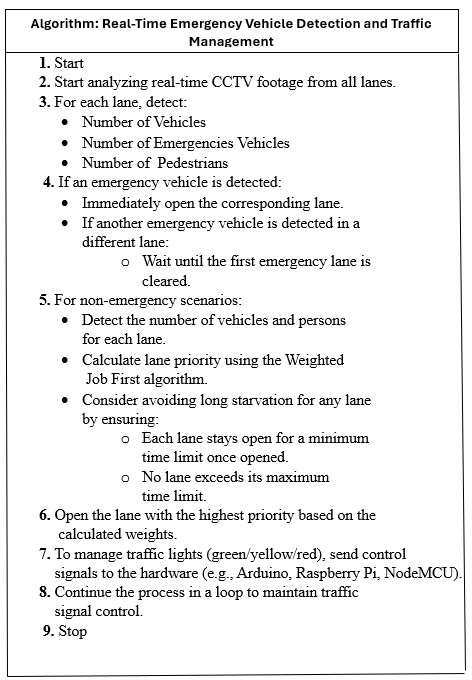
\includegraphics[width=0.9\textwidth]{figures/10.png}
    \caption{System Data Flow Diagram}
    \label{fig:data_flow}
\end{figure}

\subsection{Message Passing System}

The system uses a publish-subscribe messaging pattern:

\begin{enumerate}
    \item \textbf{Video Frames}: Camera modules publish video frames
    \item \textbf{Detection Results}: Object detection module publishes detection results
    \item \textbf{Traffic Statistics}: Traffic analysis module publishes traffic statistics
    \item \textbf{Control Commands}: Decision engine publishes control commands
    \item \textbf{Status Updates}: Hardware interface publishes status updates
\end{enumerate}

\section{Performance Optimization}

\subsection{Real-Time Processing Optimization}

Several optimization techniques are implemented for real-time performance:

\begin{enumerate}
    \item \textbf{Frame Skipping}: Processing every nth frame to reduce computational load
    \item \textbf{Region of Interest}: Focusing processing on relevant image areas
    \item \textbf{Model Quantization}: Reducing model precision for faster inference
    \item \textbf{Batch Processing}: Processing multiple frames simultaneously
    \item \textbf{Parallel Processing}: Utilizing multiple CPU cores/GPU streams
\end{enumerate}

\subsection{Memory Management}

Efficient memory management strategies:

\begin{enumerate}
    \item \textbf{Buffer Management}: Circular buffers for video frames
    \item \textbf{Memory Pooling}: Reusing allocated memory blocks
    \item \textbf{Garbage Collection}: Automatic memory cleanup
    \item \textbf{Cache Optimization}: Optimizing data access patterns
\end{enumerate}

\section{Fault Tolerance and Reliability}

\subsection{Redundancy Mechanisms}

The system implements several redundancy mechanisms:

\begin{enumerate}
    \item \textbf{Camera Redundancy}: Multiple cameras per intersection
    \item \textbf{Processing Redundancy}: Backup processing units
    \item \textbf{Communication Redundancy}: Multiple communication channels
    \item \textbf{Power Redundancy}: Uninterruptible power supply systems
\end{enumerate}

\subsection{Error Handling}

Comprehensive error handling strategies:

\begin{algorithmic}[1]
\STATE \textbf{Input:} System operation
\STATE \textbf{Output:} Error-handled operation
\STATE 
\STATE result = perform\_operation()
\IF{result == "CameraError"}
    \STATE switch\_to\_backup\_camera()
\ELSIF{result == "NetworkError"}
    \STATE switch\_to\_backup\_network()
\ELSIF{result == "ProcessingError"}
    \STATE restart\_processing\_module()
\ELSIF{result == "HardwareError"}
    \STATE activate\_fail\_safe\_mode()
\ENDIF
\end{algorithmic}

\section{Security and Privacy}

\subsection{Data Security}

The system implements robust security measures:

\begin{enumerate}
    \item \textbf{Encryption}: AES-256 encryption for data transmission
    \item \textbf{Authentication}: Multi-factor authentication for system access
    \item \textbf{Access Control}: Role-based access control mechanisms
    \item \textbf{Audit Logging}: Comprehensive logging of system activities
\end{enumerate}

\subsection{Privacy Protection}

Privacy protection measures include:

\begin{enumerate}
    \item \textbf{Data Anonymization}: Removing personally identifiable information
    \item \textbf{Selective Recording}: Recording only necessary traffic data
    \item \textbf{Automatic Deletion}: Automatic deletion of old data
    \item \textbf{Compliance}: Adherence to local privacy regulations
\end{enumerate}

\section{Scalability and Extensibility}

\subsection{Scalability Features}

The system is designed for scalability:

\begin{enumerate}
    \item \textbf{Modular Architecture}: Easy addition of new components
    \item \textbf{Distributed Processing}: Support for distributed computing
    \item \textbf{Load Balancing}: Automatic load distribution
    \item \textbf{Cloud Integration}: Optional cloud-based processing
\end{enumerate}

\subsection{Extensibility Options}

Future extension possibilities:

\begin{enumerate}
    \item \textbf{Additional Sensors}: Integration with other sensor types
    \item \textbf{Weather Integration}: Weather condition consideration
    \item \textbf{Predictive Analytics}: Traffic prediction capabilities
    \item \textbf{Mobile Applications}: Integration with mobile apps
\end{enumerate}

\section{Summary}

This chapter has presented a comprehensive system design for the machine learning and IoT-based traffic management system. The design addresses the unique challenges of traffic management in Dhaka city while providing a robust, scalable, and efficient solution. The modular architecture enables easy maintenance and future extensions, while the comprehensive security and reliability measures ensure safe and dependable operation.

The next chapter will detail the implementation aspects, including technical specifications, development processes, and deployment considerations. 